\documentclass[11pt]{article}

\usepackage[margin=1in]{geometry}
\usepackage[T1]{fontenc}
\usepackage{lmodern}
\usepackage{microtype}
\usepackage{amsmath, amssymb}
\usepackage{booktabs}
\usepackage{array}
\usepackage{tabularx}
\usepackage{tikz}
\usetikzlibrary{arrows.meta, positioning, shapes.geometric, calc, decorations.pathreplacing, backgrounds}
\usepackage{float}
\usepackage[hidelinks]{hyperref}
\usepackage{caption}
\usepackage{xcolor}
\usepackage{enumitem}
\usepackage[round]{natbib}

\setlength{\parskip}{0.5em}
\setlength{\parindent}{0pt}

\newcommand{\textub}{t_{\text{extub}}}
\newcommand{\tdeath}{t_{\text{death}}}
\newcommand{\treint}{t_{\text{reint}}}
\newcommand{\tobsend}{t_{\text{obs\_end}}}

\title{\textbf{FLAIR Task Schematic} \\[0.3em]
       Extubation Failure within 24 Hours (Task T3)}
\author{FLAIR Benchmark}
\date{\today}

\begin{document}
\maketitle

\begin{abstract}
\noindent We specify the FLAIR extubation-failure task: at the moment
of the first confirmed extubation, predict whether the patient will
accumulate less than one ventilator-free day in the next 24 hours ---
i.e., die or get reintubated. This is a one-per-stay task anchored at a
single per-hospitalization event. The interesting algorithmic
ingredient is the consensus-window IMV episode detector
(\texttt{\_ventilation\_episodes.detect\_imv\_episodes}), which
distinguishes a true extubation from sensor flicker, tracheostomy
sentinels, and intermittent ventilator swaps. Ambiguous censoring
(discharged alive less than 24h post-extubation with no observed
event) is dropped to avoid positive-unlabeled bias
\citep{epstein1997vfd, thille2011extubation}.
\end{abstract}

\section{Consensus-window IMV episode detection}
\label{sec:consensus}

A CLIF \texttt{respiratory\_support} row is a device-status sample, not
a clinical event. A single misclassified row (brief sensor disconnect,
vent swap, transient downgrade) should not be counted as intubation or
extubation. \texttt{detect\_imv\_episodes} confirms each transition
with a forward consensus window:

\begin{description}[leftmargin=2em, style=nextline]
  \item[IMV start.]
    A device $\texttt{imv}$ row at time $t$ opens an episode iff no
    contradicting non-IMV row falls in $(t,\, t + \texttt{INTUB\_WINDOW\_MIN}]$
    with $\texttt{INTUB\_WINDOW\_MIN} = 15$ minutes.

  \item[Episode close (true extubation).]
    A non-IMV row at time $t$ (while an episode is open) closes that
    episode iff no contradicting IMV row falls in
    $(t,\, t + \texttt{EXTUB\_WINDOW\_MIN}]$ with
    $\texttt{EXTUB\_WINDOW\_MIN} = 30$ minutes.

  \item[Trach sentinel.]
    A row with
    $\texttt{device\_category} = \texttt{"trach collar"}$ or
    $\texttt{tracheostomy} = \texttt{true}$ closes any open episode at
    its timestamp and halts further counting for the hospitalization.
    If the trach sentinel fires before any IMV row,
    $\texttt{is\_pre\_existing\_trach} = \texttt{true}$.
\end{description}

The detector emits one row per confirmed episode:
\texttt{(hospitalization\_id,\ episode\_index,\ episode\_start\_dttm,\
episode\_end\_dttm,\ is\_pre\_existing\_trach)}. The
$\texttt{episode\_end\_dttm}$ field is null iff the patient is still on
IMV at the end of record or the episode was closed by a trach sentinel
that did not first pass through a non-IMV transition.

\section{FLAIR operational definition}
\label{sec:def}

\subsection{Index time and label}

Let $H_i$ denote a hospitalization that survives the cohort filters
(\S\ref{sec:cohort}). Let $E^1_i = (s^1_i, e^1_i)$ be its first IMV
episode and $E^2_i = (s^2_i, e^2_i)$ its second (if any).

\begin{description}[leftmargin=2em, style=nextline]

\item[Prediction time ($\textub^i$).]
$\textub^i = e^1_i =$ \texttt{episode\_end\_dttm} of the first episode.
Exactly one decision point per hospitalization
(\emph{one-per-stay}).

\item[Reintubation time.]
$\treint^i = s^2_i$ if $E^2_i$ exists, $+\infty$ otherwise.

\item[Death time.]
$\tdeath^i$ from \texttt{hospitalization.death\_dttm}; $+\infty$ if
null.

\item[Label horizon.]
$(\textub^i,\, \textub^i + 24\text{h}]$.

\item[Label (\texttt{label\_extubation\_failure\_24h}).]
\[
y_i \;=\; \mathbb{1}\!\left[
  \tdeath^i \in (\textub^i,\, \textub^i + 24\text{h}\,]
  \;\;\vee\;\;
  \treint^i \in (\textub^i,\, \textub^i + 24\text{h}\,]
\right].
\]

\item[Observability end.]
$\tobsend^i = \texttt{coalesce}(\tdeath^i,\, t^{\text{disch}}_i)$.

\item[Censoring drop.]
Keep row iff
\[
\tdeath^i \in (\textub^i,\, \textub^i + 24\text{h}\,]
\;\;\vee\;\;
\treint^i \in (\textub^i,\, \textub^i + 24\text{h}\,]
\;\;\vee\;\;
\tobsend^i \;\geq\; \textub^i + 24\text{h}.
\]
A patient discharged alive less than 24 hours after extubation with no
observed death or reintubation has \emph{unobserved} outcome; treating
that as $y_i = 0$ would inject positive-unlabeled bias.

\end{description}

\subsection{Cohort}
\label{sec:cohort}

\begin{itemize}[leftmargin=2em]
  \item Age at admission $\ge 18$ with valid \texttt{admission\_dttm}
        and \texttt{discharge\_dttm}.
  \item $\geq 1$ ICU ADT record.
  \item First IMV episode ($\texttt{episode\_index} = 1$) has
        non-null \texttt{episode\_end\_dttm} (i.e., a confirmed
        extubation exists per \S\ref{sec:consensus}).
  \item \textbf{Exclude} pre-existing tracheostomy
        (\texttt{is\_pre\_existing\_trach}).
  \item \textbf{Exclude} first episode closed by a trach sentinel
        ($\pm 1$min tolerance via
        \texttt{TRACH\_CLOSURE\_TOLERANCE\_MIN} $= 1$;
        \texttt{\_drop\_trach\_closed} in
        \texttt{task3\_extubation\_failure\_24h.py}).
  \item \textbf{Exclude} ambiguous censoring (discharged alive
        $<24$h post-extubation with no death and no reintubation).
\end{itemize}

\subsection{CLIF tables and categories used}
\label{sec:t3-clif}

Task~T3 reads four CLIF v2.1 tables. The cohort entry filter is on
\texttt{adt.location\_category}; the index event itself is derived from
two category-column predicates in \texttt{respiratory\_support}.

\begin{table}[H]
\centering
\small
\begin{tabular}{@{}llp{7.0cm}@{}}
\toprule
\textbf{CLIF table} & \textbf{Category column} & \textbf{Literal values kept (case-insensitive)} \\
\midrule
\texttt{hospitalization}    & ---                       & cohort/demographics join; no category filter \\
\texttt{patient}            & ---                       & demographics join; no category filter \\
\texttt{adt}                & \texttt{location\_category} & $\{\texttt{"icu"}\}$ \\
\texttt{respiratory\_support} & \texttt{device\_category} &
$\{\texttt{"imv"}\}$ classifies a row as IMV; any other value is
non-IMV; \\
& \multicolumn{2}{l}{$\;\;$ trach sentinel: \texttt{device\_category} $=$
\texttt{"trach collar"} $\vee$ \texttt{tracheostomy} $=$ \texttt{true}$^{\dagger}$} \\
\bottomrule
\end{tabular}
\caption{CLIF surface for Task~T3. Both the IMV-vs-non-IMV classifier
and the trach sentinel live in \texttt{respiratory\_support}; the
consensus-window logic of \S\ref{sec:consensus} runs on top of these
two predicates.}
\end{table}

$\dagger$ \texttt{tracheostomy} is a \emph{boolean} column, not a
category. The trach sentinel fires when either the categorical
\texttt{device\_category} equals \texttt{"trach collar"} OR the boolean
\texttt{tracheostomy} is \texttt{true}. A site whose CLIF
\texttt{respiratory\_support} export omits one of these signals can
still detect tracheostomies via the other; sites that omit both will
silently include trach-decannulation events in the extubation cohort.

Columns selected from each table:
\begin{itemize}[leftmargin=2em, itemsep=0pt]
  \item \texttt{hospitalization}: \texttt{hospitalization\_id},
        \texttt{patient\_id}, \texttt{admission\_dttm},
        \texttt{discharge\_dttm}, \texttt{age\_at\_admission},
        \texttt{discharge\_category} (loaded but not filtered).
  \item \texttt{patient}: \texttt{patient\_id},
        \texttt{sex\_category}, \texttt{race\_category},
        \texttt{ethnicity\_category}, \texttt{death\_dttm}.
  \item \texttt{adt}: \texttt{hospitalization\_id},
        \texttt{location\_category}, \texttt{in\_dttm},
        \texttt{out\_dttm}.
  \item \texttt{respiratory\_support}: \texttt{hospitalization\_id},
        \texttt{recorded\_dttm}, \texttt{device\_category},
        \texttt{tracheostomy}.
\end{itemize}

\section{Algorithmic flow}
\label{sec:flow}

\begin{figure}[H]
\centering
% Algorithmic flowchart for FLAIR extubation-failure-24h task build pipeline.

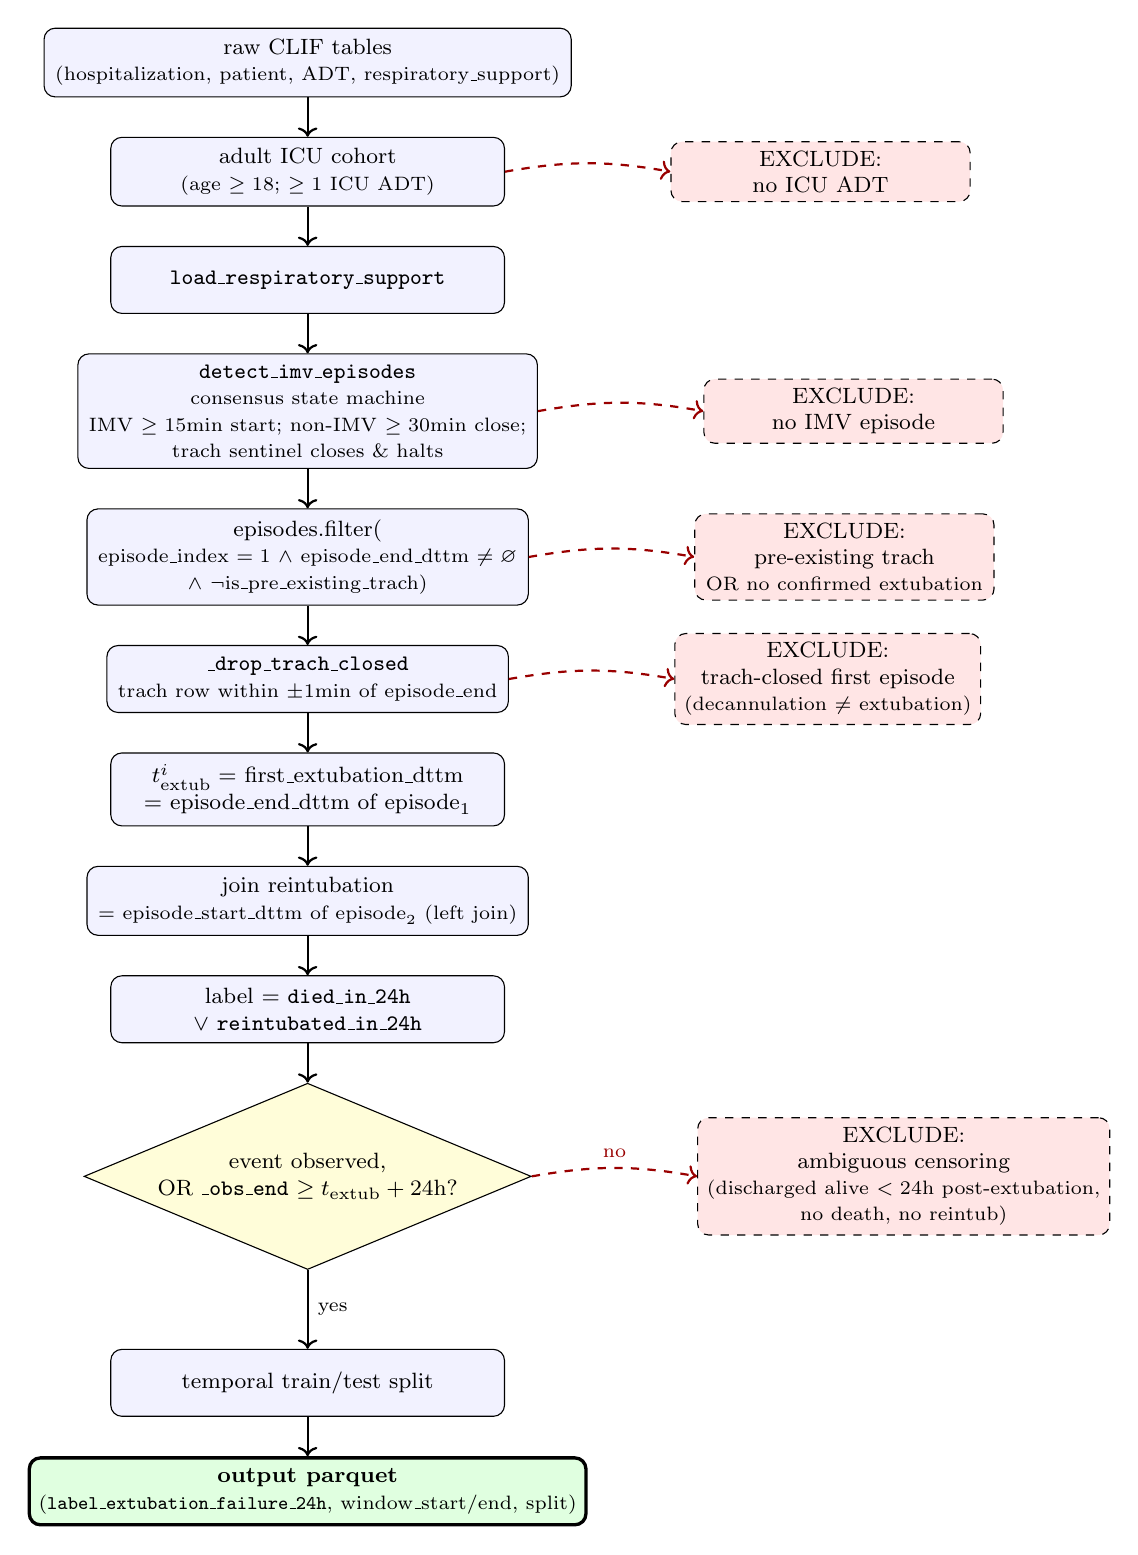
\begin{tikzpicture}[
    node distance=0.5cm and 0.7cm,
    every node/.style={font=\footnotesize, align=center},
    box/.style={draw, rounded corners, fill=blue!5,
                minimum width=5.0cm, minimum height=0.85cm, inner sep=4pt},
    dbox/.style={draw, diamond, aspect=2.4, fill=yellow!15,
                 minimum width=4.4cm, inner sep=2pt},
    excl/.style={draw, rounded corners, fill=red!10, dashed,
                 minimum width=3.8cm, minimum height=0.7cm},
    outbox/.style={draw, rounded corners, fill=green!12, very thick,
                minimum width=5.0cm, minimum height=0.85cm},
    arrow/.style={->, thick},
    sidearrow/.style={->, thick, red!60!black, dashed},
]
    % main pipeline
    \node[box] (raw)
        {raw CLIF tables\\\scriptsize(hospitalization, patient, ADT, respiratory\_support)};
    \node[box, below=of raw] (cohort)
        {adult ICU cohort\\\scriptsize(age $\geq 18$; $\geq 1$ ICU ADT)};
    \node[box, below=of cohort] (loadresp)
        {\texttt{load\_respiratory\_support}};
    \node[box, below=of loadresp] (detect)
        {\texttt{detect\_imv\_episodes}\\\scriptsize consensus state machine\\
         \scriptsize IMV $\geq 15$min start; non-IMV $\geq 30$min close;\\
         \scriptsize trach sentinel closes \& halts};
    \node[box, below=of detect] (filter)
        {episodes.filter(\\\scriptsize episode\_index $= 1\ \wedge$
         episode\_end\_dttm $\neq\varnothing$\\\scriptsize
         $\wedge\ \neg$is\_pre\_existing\_trach)};
    \node[box, below=of filter] (trach)
        {\texttt{\_drop\_trach\_closed}\\\scriptsize trach row within
         $\pm 1$min of episode\_end};
    \node[box, below=of trach] (pred)
        {$\textub^i =$ first\_extubation\_dttm\\$= $
         episode\_end\_dttm of $\text{episode}_1$};
    \node[box, below=of pred] (reint)
        {join reintubation\\\scriptsize $=$ episode\_start\_dttm of
         $\text{episode}_2$ (left join)};
    \node[box, below=of reint] (lab)
        {label $=$ \texttt{died\_in\_24h}\\
         $\vee$ \texttt{reintubated\_in\_24h}};

    \node[dbox, below=of lab] (decide)
        {event observed,\\OR \texttt{\_obs\_end} $\geq \textub + 24$h?};

    \node[box, below=1.0cm of decide] (split)
        {temporal train/test split};
    \node[outbox, below=of split] (parquet)
        {\textbf{output parquet}\\\scriptsize{(\texttt{label\_extubation\_failure\_24h},
         window\_start/end, split)}};

    % exclusions on the right
    \node[excl, right=2.1cm of cohort] (exclNoIcu)
        {EXCLUDE:\\no ICU ADT};
    \node[excl, right=2.1cm of detect] (exclNoImv)
        {EXCLUDE:\\no IMV episode};
    \node[excl, right=2.1cm of filter] (exclPre)
        {EXCLUDE:\\pre-existing trach\\\scriptsize OR no confirmed
         extubation};
    \node[excl, right=2.1cm of trach] (exclTrach)
        {EXCLUDE:\\trach-closed first episode\\\scriptsize
         (decannulation $\neq$ extubation)};
    \node[excl, right=2.1cm of decide] (exclAmb)
        {EXCLUDE:\\ambiguous censoring\\\scriptsize(discharged alive
         $< 24$h post-extubation,\\\scriptsize no death, no reintub)};

    % main arrows
    \draw[arrow] (raw) -- (cohort);
    \draw[arrow] (cohort) -- (loadresp);
    \draw[arrow] (loadresp) -- (detect);
    \draw[arrow] (detect) -- (filter);
    \draw[arrow] (filter) -- (trach);
    \draw[arrow] (trach) -- (pred);
    \draw[arrow] (pred) -- (reint);
    \draw[arrow] (reint) -- (lab);
    \draw[arrow] (lab) -- (decide);
    \draw[arrow] (decide) -- node[right, font=\scriptsize]{yes} (split);
    \draw[arrow] (split) -- (parquet);

    % exclusion arrows
    \draw[sidearrow] (cohort.east) to[bend left=10] (exclNoIcu.west);
    \draw[sidearrow] (detect.east) to[bend left=10] (exclNoImv.west);
    \draw[sidearrow] (filter.east) to[bend left=10] (exclPre.west);
    \draw[sidearrow] (trach.east) to[bend left=10] (exclTrach.west);
    \draw[sidearrow] (decide.east) to[bend left=10]
        node[above, font=\scriptsize]{no} (exclAmb.west);

\end{tikzpicture}

\caption{Build pipeline for Task~T3. Solid arrows: main flow. Dashed
red arrows: exclusions. The diamond enforces the censoring rule: any
hospitalization whose observation window closes before
$\textub^i + 24\text{h}$ without an observed death or reintubation is
dropped, since its label is unobservable.}
\label{fig:t3-flow}
\end{figure}

Step-by-step prose:

\begin{enumerate}[leftmargin=2em]
  \item Load CLIF tables: \texttt{hospitalization}, \texttt{patient},
        \texttt{adt}, \texttt{respiratory\_support}.
  \item Apply adult-ICU cohort filters.
  \item \texttt{load\_respiratory\_support(cfg, hosp\_ids)} returns all
        device-status rows for the cohort.
  \item Run \texttt{detect\_imv\_episodes(resp)} (\S\ref{sec:consensus}).
  \item Filter to first episodes that ended in a confirmed extubation:
        $\texttt{episode\_index} = 1\ \wedge$ \texttt{episode\_end\_dttm}
        $\neq \varnothing\ \wedge\ \neg$\texttt{is\_pre\_existing\_trach}.
  \item Drop trach-closed first episodes via
        \texttt{\_drop\_trach\_closed}: any first episode whose
        \texttt{episode\_end\_dttm} coincides with a
        \texttt{trach collar} or \texttt{tracheostomy=true} row within
        $\pm 1$ minute is removed (decannulation $\neq$ extubation).
  \item Extract second-episode starts as
        $\treint^i = $ \texttt{episode\_start\_dttm} where
        $\texttt{episode\_index} = 2$ (left join; null if none).
  \item Join hospitalization-level $\tdeath^i$ and $t^{\text{disch}}_i$.
  \item Compute $y_i = \texttt{\_died}\ \vee\ \texttt{\_reintub}$ per
        the formulas above.
  \item Drop ambiguous censoring rows (the diamond in
        Figure~\ref{fig:t3-flow}).
  \item Set \texttt{window\_start} $= \textub^i - 24$h,
        \texttt{window\_end} $= \textub^i$ (fixed 24h lookback).
  \item Apply temporal train/test split via
        \texttt{flair\_benchmark.\_split.assign\_split}, keyed on
        $\textub^i$.
  \item Select \texttt{OUTPUT\_COLS} and persist as parquet.
\end{enumerate}

\section{Design choices and rationale}
\label{sec:rationale}

\paragraph{Why 15-minute / 30-minute consensus windows.}
RespiratorySupport in CLIF is a device-status sample: brief sensor
dropouts, vent swaps, and transient downgrades produce single rows
that look like state transitions but are not. The 15-minute IMV
consensus on the start side and the 30-minute non-IMV consensus on the
close side filter these artifacts while still resolving real
extubations within a clinically reasonable margin. The asymmetric
choice (15 in, 30 out) reflects the asymmetric cost: a missed
intubation start would lose only a small slice of input-feature
window, whereas a false extubation close anchors the entire label.

\paragraph{Why drop trach-closed first episodes.}
The state machine treats a trach sentinel as an episode close so the
counting can halt cleanly, but a tracheostomy decannulation is not the
clinical event this task predicts. Modeling it as an extubation would
mix a planned airway management procedure with the unplanned
reintubation-vs-failure decision and inflate the cohort with patients
whose 24h outcome is dominated by trach-specific physiology rather
than spontaneous-breathing readiness.

\paragraph{Why drop ambiguous censoring.}
A patient extubated at 03:00 and discharged at 18:00 the same day with
no death and no reintubation has only 15 hours of post-extubation
observability. Labeling them $y_i = 0$ would treat the absence of
observed failure as evidence of success when it is just censoring.
This is a textbook positive-unlabeled trap; the cohort filter resolves
it by dropping the unobservable row entirely. The cost is a small
positive-skew in the retained cohort (patients with longer
post-extubation observation are slightly sicker on average), which the
main paper's Discussion acknowledges.

\paragraph{Why one-per-stay (not continuous).}
The decision to extubate is itself the clinical handle. Predictions at
arbitrary timesteps before the actual extubation are not actionable
because they would be evaluated against a different intervention
(extubation at a different time). Restricting to the actual
extubation moment makes the label well-defined and the comparison
across hospitalizations meaningful.

\paragraph{Prevalence implications.}
MIMIC-CLIF: 26{,}771 extubation episodes pass the cohort filters,
1{,}456 positive (5.4\%; see \texttt{docs/paper/outline.tex} Table~1).
Reporting AUPRC alongside AUROC is mandatory.

\section{Out of scope}

\begin{itemize}[leftmargin=2em]
  \item Second-, third-, and later-extubation decision points.
  \item Non-invasive-ventilation (NIV) as a failure mode (currently
        only death and reintubation count).
  \item A continuous variant that predicts extubation failure ahead of
        the actual extubation.
  \item Curated drug-list or ventilator-mode feature design.
\end{itemize}

\bibliographystyle{plainnat}
\bibliography{references}

\end{document}
